\section{Listen}

Eine Liste ist eine dynamische Datenstruktur.
Arrays im genegsatz dazu sind statische Datenstrukturen.
Listenelemente werden mittels Pointer verbunden.

\textbf{Achtung!} List \lstinline[style=cppstyle]|search| sollte nicht bei \lstinline[style=cppstyle]|double| verwendet werden, da wegen der Rundungsfehler nicht immer das richtige Element gefunden wird. Braucht ein delta!

\subsection{Einfach verkettete Liste}
Die Pointerverbindung geht nur in eine Richtung.

\begin{lstlisting}[style=cppstyle]
struct Node {
	Item
	value;
	Node* next;
};
\end{lstlisting}

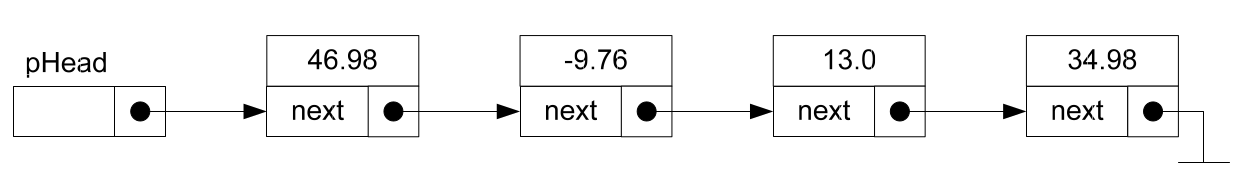
\includegraphics[width=\linewidth]{"Images/single_linked_list.png"}


Bonderer: Dann muss ich den Vorderen und Hinteren noch richtig durchnehmen.

\subsection{Doppelt verkettete Liste}
\begin{lstlisting}[style=cppstyle]
struct Node {
	Item
	value;
	Node* next;
	Node* prev;
};
\end{lstlisting}

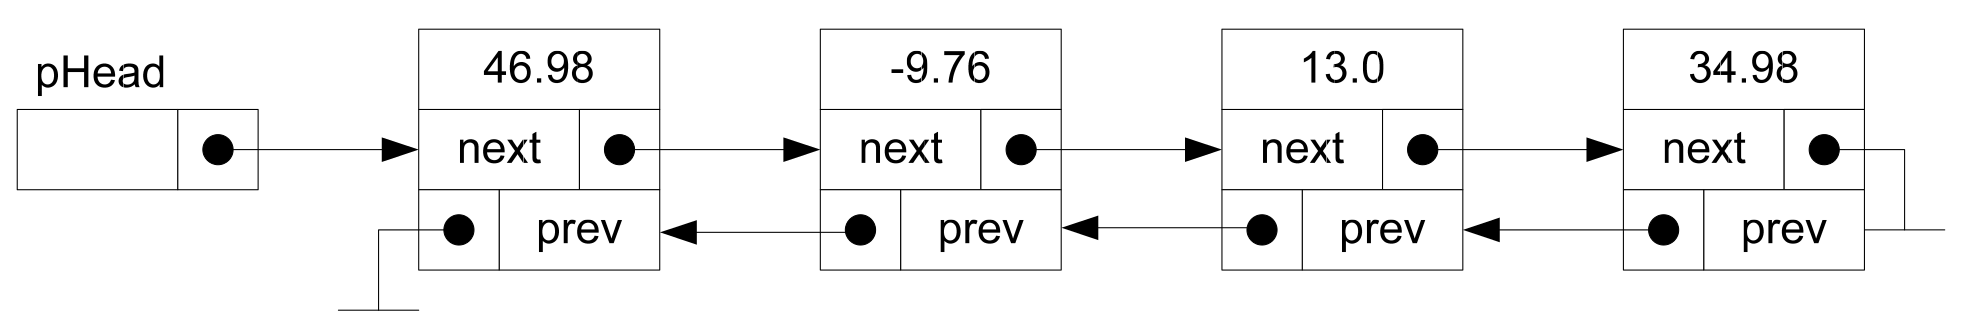
\includegraphics[width=\linewidth]{"Images/double_linked_list.png"}